\documentclass[border=10pt]{standalone}

\usepackage{tikz}
\usepackage{tikzsymbols}
\usetikzlibrary{calc,patterns,shapes.geometric}

\def\centerarc[#1](#2)(#3:#4:#5){\draw[#1] ($(#2)+({#5*cos(#3)},{#5*sin(#3)})$) arc (#3:#4:#5);}

\begin{document}
	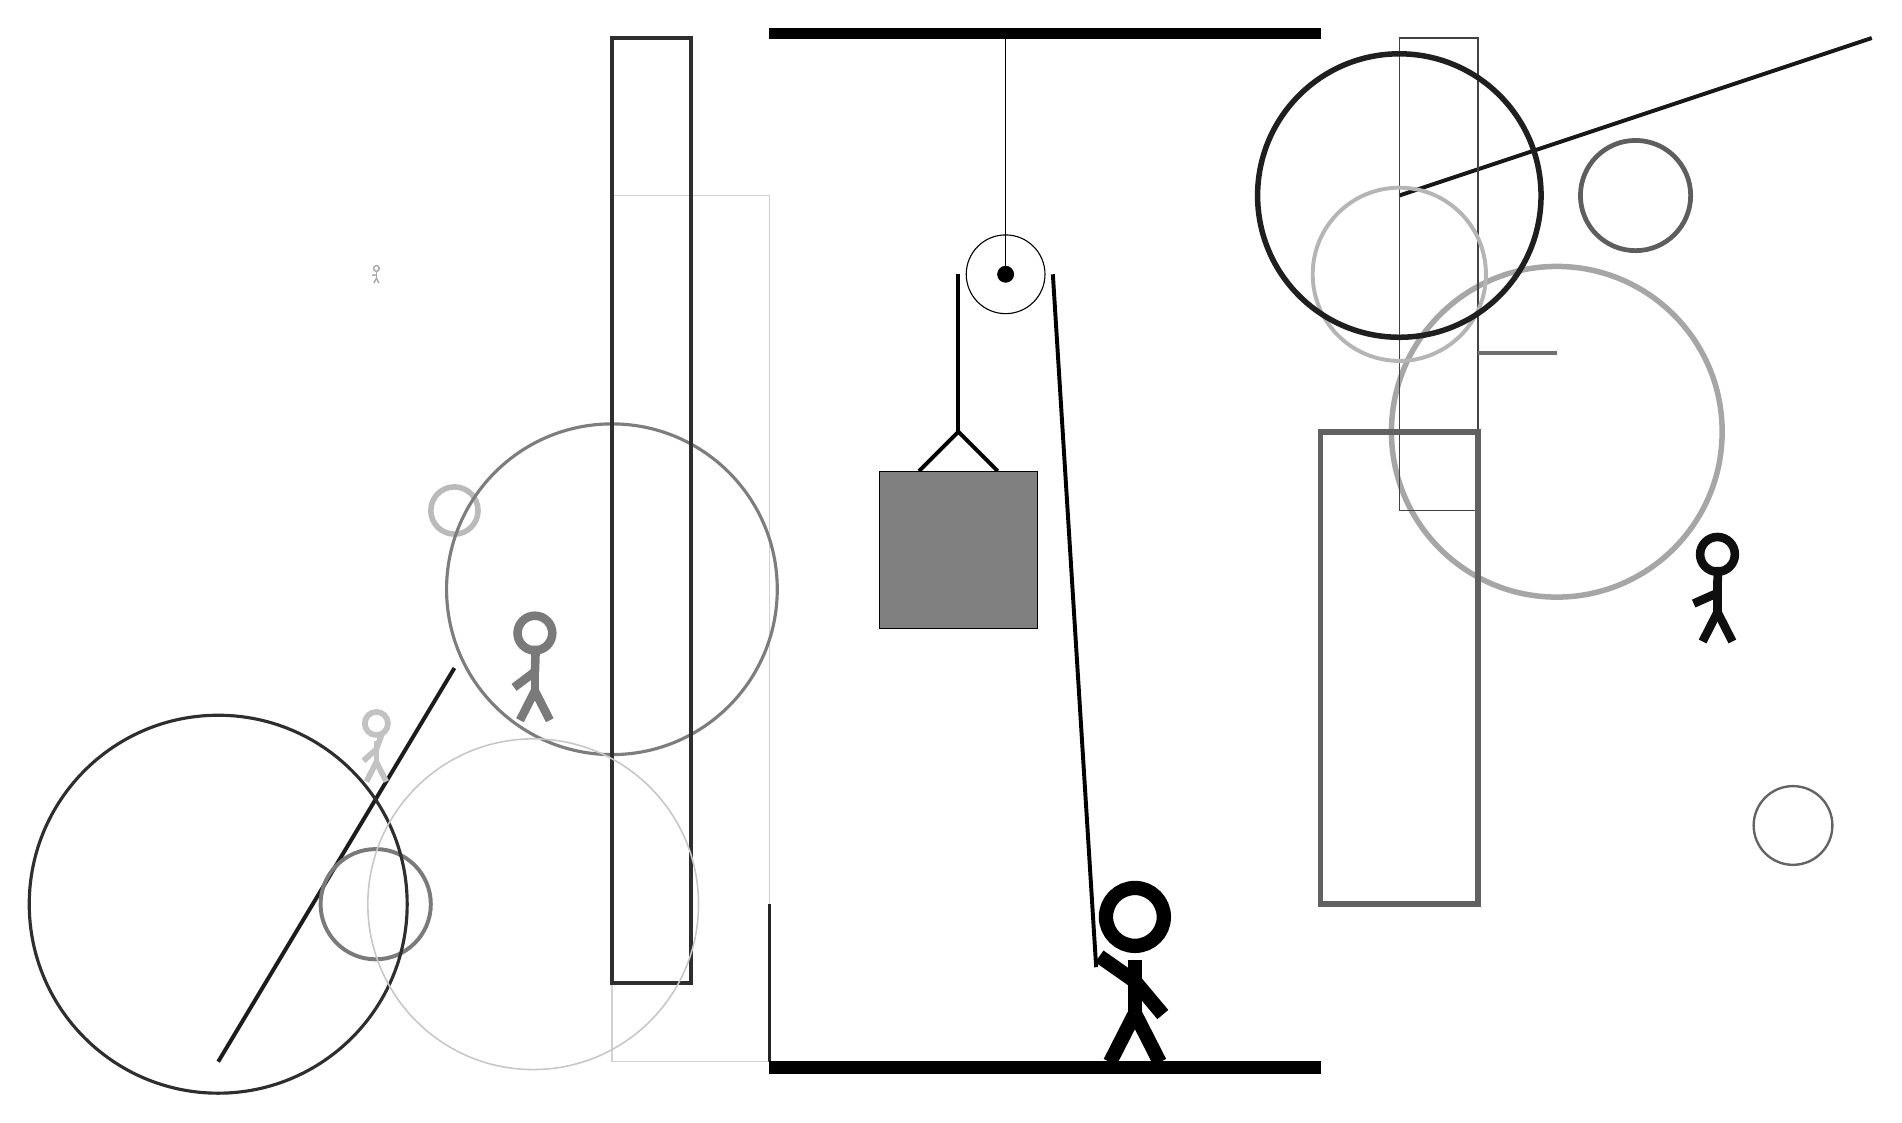
\begin{tikzpicture}
		%%%%% START %%%%%
		
		\draw[fill=black] (-2, 10) rectangle (5, 10.125);
		
		\draw (1, 7) circle (0.5);
		\draw[fill=black] (1, 7) circle (0.1);
		\draw (1, 10) -- (1, 7);
		
		\draw[line width=0.5mm] (-0.1, 4.5) -- (0.4, 5.0) -- (0.9, 4.5);
		\draw[fill=black!50] (-0.6, 4.5) rectangle (1.4, 2.5);
		
		\draw[line width=0.5mm] (0.4, 7) -- (0.4, 5.0);
		\centerarc[line width=0.5mm](1, 7)(0:180:0.6);
		\draw[line width=0.5mm](1.6, 7) -- (2.15, -1.8);
		
		\draw [line width=0.7mm, color=black!27](-6, 4) circle (0.3);
		
		\draw [line width=0.7mm, color=black!35](8, 5) circle (2.1);
		\draw[line width=0.5mm, color=black!89](-6, 2) -- (-9, -3);
		\draw[line width=0.2mm, color=black!18] (-4, -3) rectangle (-2, 8);
		\draw [line width=0.6mm, color=black!63](9, 8) circle (0.7);
		\draw [line width=0.5mm, color=black!52](-7, -1) circle (0.7);
		\draw [line width=0.3mm, color=black!61](11, 0) circle (0.5);
		\draw [line width=0.4mm, color=black!51](-4, 3) circle (2.1);
		\draw[line width=0.5mm, color=black!91](6, 8) -- (12, 10);
		\draw[line width=0.2mm, color=black!74] (6, 10) rectangle (7, 4);
		\draw [line width=0.5mm, color=black!29](6, 7) circle (1.1);
		
		\draw[line width=0.5mm, color=black!82] (-3, -2) rectangle (-4, 10);
		\node[line width=0.2mm, color=black!52] at (-5, 2) {\Strichmaxerl[6][37][88]};
		
		\node[line width=0.3mm, color=black!34] at (-7, 7) {\Strichmaxerl[1][5][90]};
		\draw[line width=0.4mm, color=black!56] (7, 6) rectangle (8, 6);
		\draw [line width=0.7mm, color=black!88](6, 8) circle (1.8);
		
		\node[line width=0.2mm, color=black!94] at (10, 3) {\Strichmaxerl[6][24][89]};
		\draw [line width=0.4mm, color=black!82](-9, -1) circle (2.4);
		\draw[line width=0.7mm, color=black!62] (5, 5) rectangle (7, -1);
		\draw [line width=0.2mm, color=black!22](-5, -1) circle (2.1);
		\draw[line width=0.4mm, color=black!86] (-2, -1) rectangle (-2, -3);
		\node[line width=0.3mm, color=black!24] at (-7, 1) {\Strichmaxerl[4][42][70]};
		
		
		\node at (2.6, -1.9) {\Strichmaxerl[10][-35][-50]};
		
		\draw[fill=black] (-2, -3) rectangle (5, -3.15);
		
		%%%%% END %%%%%
	\end{tikzpicture}
\end{document}